\documentclass[10pt,twocolumn,letterpaper]{article}
\usepackage{graphicx}
\usepackage{amsmath}
\usepackage{amssymb}
\usepackage{booktabs}
\usepackage{nicefrac}
\usepackage{algorithm}
\usepackage[algo2e]{algorithm2e} 
\usepackage{multirow}
\usepackage[pagebackref,breaklinks,colorlinks]{hyperref}

% Support for easy cross-referencing
\usepackage[capitalize]{cleveref}
\crefname{section}{Sec.}{Secs.}
\Crefname{section}{Section}{Sections}
\Crefname{table}{Table}{Tables}
\crefname{table}{Tab.}{Tabs.}

\begin{document}
\nocite{*}

\title{Exam 13/12/2022}
\author{Philippe Schartier}
\maketitle

\begin{figure}[H]
    \centering
    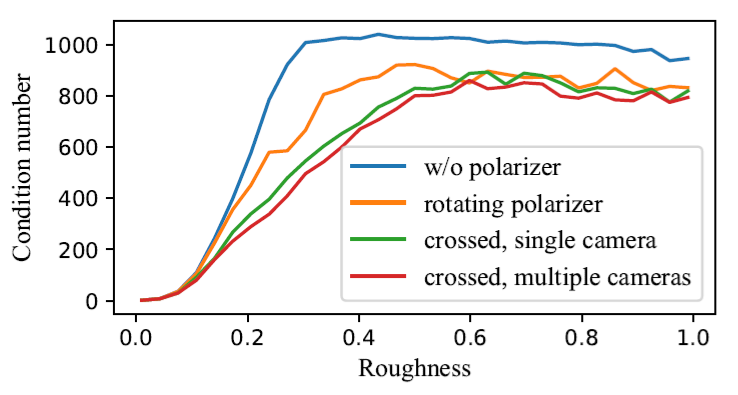
\includegraphics[width=6cm]{image/image1.PNG}
    \caption{Figure 6: Condition number with respect to the roughness
of the wall. Lower the better. The roughness ranges 0
(mirror-like) to 1 (diffuse-like). Our method has the lowest
condition number for all roughness parameter.}
    \label{fig:figure1}
\end{figure}

Although the plots of single and multiple cameras look similar,
we observe that the multiple camera setting is always
slightly better than single camera setting. When the roughness
decreases, the wall becomes mirror-like and there is no
improvement using a polarizer because the NLOS scene is
originally visible. The best performance is observed at the
middle of specular and diffuse reflections, where a lot of
materials have such specularities [30].

\section{\label{sec : Experiment} Experiment}

Real experiments are consistent with simulations: polarization
improves NLOS image reconstruction. For all following
experiments, we use ADMM to solve Eq. (2), consisting
of a 2D total variation regularizer with a box constraint.
For clarity, we estimate

\begin{equation}
    \mathbf{Î}= argmin || \textbf{i - Ti} ||^2_2 + \lambda \textit{TV}_2_D 
    \label{eq:eq1}
\end{equation}
\begin{equation}
    s. t.  0$\geq$1$\geq$1.
    \label{eq:eq2}
\end{equation}

Because this is a convex optimization problem, it can be
solved in a polynomial time. For all cases, the BRDF of the
wall is measured beforehand.Polarized NLOS Firstly, we evaluate the polarized NLOS
without partial occluder. For numerical evaluation of nonpolarized
scene, a projector is used to project the scene image.
\cref{fig:figure1} shows the setup and the result. Two images
are compared with and without the polarizer in front of the
camera. While it is difficult to see the projected scenes if
the polarizer is not used, the scene is visible using the polarizer.
We also projected more images, which can be found
in the supplementary material. The table shows the numerical
evaluation of the results. Peak signal to noise ration
(PSNR), zero-mean normalized cross correlation (ZNCC),
and structural similarity (SSIM) are used. It is confirmed

\begin{figure}[H]
    \centering
    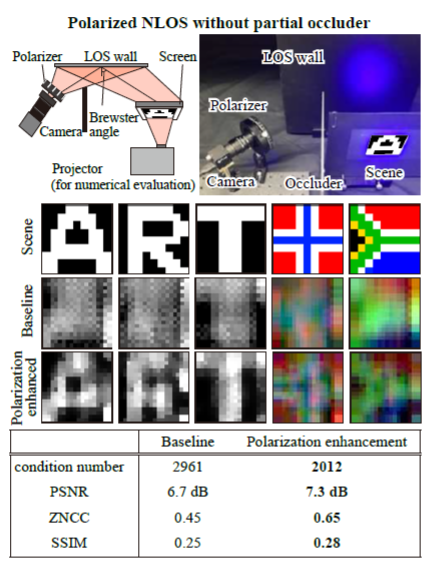
\includegraphics[width=6cm]{image/image4.PNG}
    \caption{Figure 7: Polarized NLOS results without occluder. A
projector is used for numerical evaluation and to make the
scene unpolarized. The scene is recovered with and without
the polarizer in front of the camera. Using polarization, the
recovered images are improved. Improvement is confirmed
by comparing condition number and three image measures.}
    \label{fig:figure2}
\end{figure}


that the condition number is decreased and the recovered
image is improved for every image metric if the polarization
is used.
Polarized NLOS w/ partial occluder for reflective objects
Here, we show that Polarized NLOS can also enhance
existing techniques. As shown in \cref{fig:figure3} \textit{top-left},
we reproduce the partial occluder method from Saunders et
\textit{et al.} [39]. Reflective object scenes are recovered in this experiment
and enhanced by polarization. \cref{fig:figure3} shows the
setup, the target object, the recovered result by the existing
method, and the enhanced result by polarization. The target
object is lit by an uncontrolled light source. In the results
of the baseline method, it is difficult to see the resolution
chart and the content of the book. On the other hand, our
technique recovers images with higher contrast. The clear
texture of resolution chart and printed materials are visualized
in detail. The observed image is 160 × 100 pixels and

\begin{figure}[H]
    \centering
    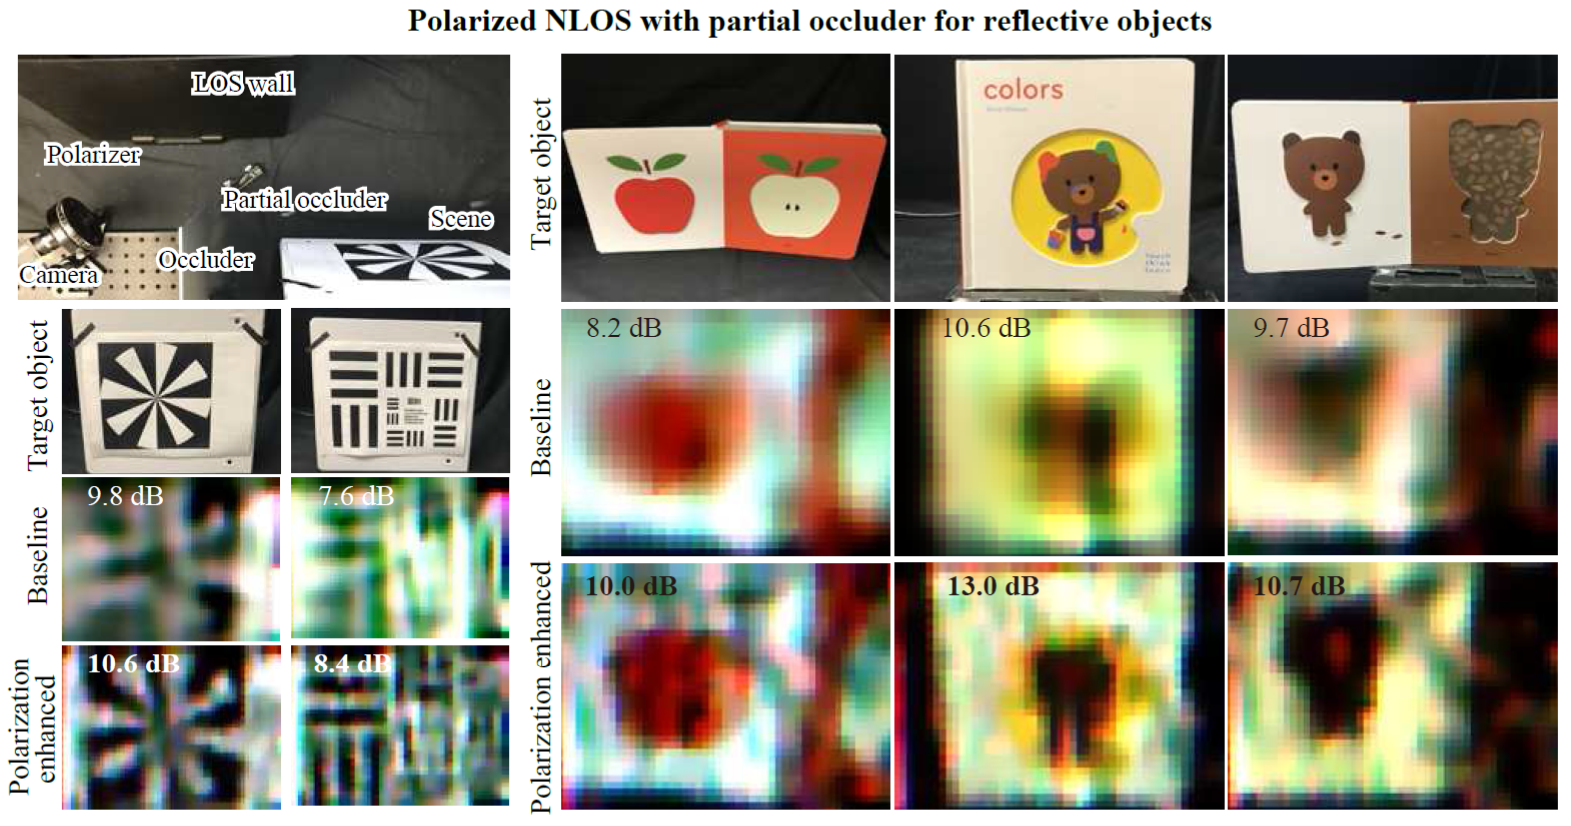
\includegraphics[width=6cm]{image/image3.PNG}
    \caption{Figure 8: Results for reflective objects. Top-left: the setting of the experiment. The scene is a reflective object (not selfluminous).
1st row: The photograph of target objects. 2nd row: The recovered images by the baseline method [39]. Bottom
row: The recovered images by our method. High frequency details are recovered. Clear detail of resolution charts, sharp edge
of apple, and the detailed shape of bears are clearly visualized. PSNR values are calculated with homography-transformed
photograph for reference.}
    \label{fig:figure3}
\end{figure}

the scene is 56 × 40 pixels, so the matrix is 16000 × 2240.
The exposure is 5 seconds. The processing time to solve \cref{eq:eq1} takes approximately 1.5 seconds. Our method quantitatively
and qualitatively improves the reconstruction. We
provide more diverse scenes in the supplement.

Comparing our enhancement to image processing An
interesting question that is raised is whether the performance
improvements we obtain could be achieved by applying
image post-processing algorithms to conventional
NLOS (without polarization). Figure 9 shows the result of
projected images and also includes the result of applying
image post-processing. The baseline method in this case is
[39]. Here, a total variation (TV) denoising algorithm [7]2
and a deep learning image processor (neural enhance) [1]
are used. While the image is improved by post processing,
it is impossible to recover the higher frequency component
that is lost on the wall reflection, because recovering lost information
is mathematically impossible. On the other hand,
our method recovers higher frequency detail, which is preserved
by polarization light transport. PSNR, ZNCC, and SSIM values show significant improvement.

\section{\label{sec : Discussion} Discussion}


In summary, there are two surprising findings from this
paper. \textit{The first surprising finding} is that polarized NLOS
has superior results to ordinary NLOS. The finding is a surprise
as initially we were not sure if any method could overcome
the 50 light loss inherent to using a polarization filter.
We are cautiously optimistic, now that this paper has
surpassed the break-even point by a considerable margin.
\textit{The second surprising finding} is that our polarization paper
does not actually leverage the rotation angle of the polarizing
filter. In contrast, we use the principle of leakage,
observed when one views an liquid crystal display off-axis.
Our method is not without assumptions, though our practical
results substantiate the validity of our assumptions. For
instance, we assume that the wall preserves polarization.
This holds for many rough surfaces, although for certain
surfaces the signal can be subtle. Concretely, walls that
have a dominant subsurface scattering, such as plastic and
plaster, can be more challenging because one loses the polarization
property, i.e., the ratio of polarization due to Fresnel
reflection becomes low. In the future, we might seek to

{\small
\bibliographystyle{IEEEtran}
\bibliography{references}
}

\end{document}
